\subsection{Funktionsweise}
\label{subsec:poffunktionsweise}

Informationen werden mittels Intensitätsmodulationen der Lichtstrahlen
übertragen. Dabei wird das Licht durch eine transparente Kern, welcher von einem
Mantel umgeben ist, gesendet (siehe \autoref{fig:pofprinzip}). Die Brechzahl $n$
des Kernes ist dabei größer als die des Mantels. Dies ermöglicht eine
Totalreflexion des Lichts am Übergang von Kern zum Mantel.
\autoref{fig:poflichtausbreitung} zeigt zwei mögliche Ausbreitungen von
Lichtimpulsen in einer polymer optischen Faser. Die Laufzeiten der beiden
Strahlen untrscheidet sich jedoch, da der hellblaue Strahl einen kürzeren Weg
für die Durchquerung des abgebildeten Leiterstückes als der grüne Strahl
zurücklegt. Die Laufzeitunterschied zwischen den Lichtstrahlen beschränken die
Bandbreite des Kabels. Die Bitraten erhöhen sich bei kürzeren Strecken, da sich
die Unterschiede zwischen den Laufzeiten verringern. Durch die Totalreflektion
kann das Licht auch durch Biegungen geleitet werden. \cite{pofacprinzip}

%Die Laufzeitunterschied zwischen dem schnellsten Strahl (ohne eine Reflektion) und dem langsamsten Strahl (die meistes Reflektion\footnote{Die Totalreflexion ist ab einem bestimmten Einfallswinkel nicht mehr möglich. Dadurch wird die maximale Reflexionszahl auf einer gewissen Strecke beschränkt}) bestimmt die Bandbreite des Kabels.

%TODO: Explain "Totalreflexion"

\begin{figure}[h]
    \begin{center}
        \begin{minipage}[t]{0.4\textwidth}
            \begin{center}
                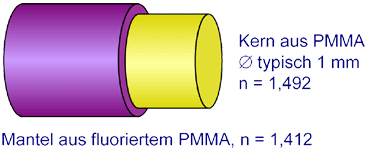
\includegraphics[height=0.4\textwidth]{Bilder/Optische_Wellenleiter_Die_Polymer_Optische_Faser/Funktionsweise/pofprinzip.png}
                \caption[Aufbau eines Kabels aus POF \newline \url{http://www.pofac.fh-nuernberg.de/pofac/de/was_sind_pof/images/pof_prinzip.png}]{Aufbau eines Kabels aus POF}
                \label{fig:pofprinzip}
            \end{center}
        \end{minipage}
        \hspace{0.025\textwidth}
        \begin{minipage}[t]{0.4\textwidth}
            \begin{center}
                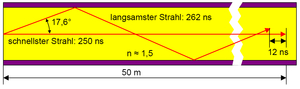
\includegraphics[height=0.1\textheight]{Bilder/Optische_Wellenleiter_Die_Polymer_Optische_Faser/Funktionsweise/poflichtausbreitung.png}
                \caption[Ausbreitung von Licht in einem optischen Wellenleiter \newline \url{http://www.itwissen.info/bilder-klein/lwl-mit-verschiedenen-moden.png}]{Ausbreitung von Licht in einem optischen Wellenleiter} %TODO: better resolution
                \label{fig:poflichtausbreitung}
            \end{center}
        \end{minipage}
    \end{center}
\end{figure}

\autoref{fig:pofdaempfung} zeigt die Dämpfungsfenster einer polymer optischen
Faser. Diese liegen bei den Farben grün, gelb und rot. Um die Intensitätsabnahme
möglichst gering zu halten und damit die Reichweite zu erhöhen werden
Wellenlängen für die Lichtimpulse gewählt, die in den Dämpfungsfenstern
liegen. Als Lichtquelle kann zum Beispiel eine LED verwendet
werden. \cite{pofacsi} %TODO: Picture of LED

\begin{figure}[h]
    \begin{center}
        \begin{minipage}[t]{0.4\textwidth}
            \begin{center}
                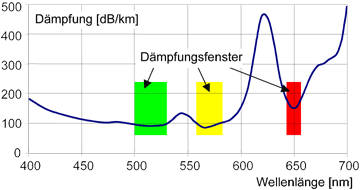
\includegraphics[height=0.1\textheight]{Bilder/Optische_Wellenleiter_Die_Polymer_Optische_Faser/Funktionsweise/pofdaempfung.png}
                \caption[Dämpfungsfenster bei einer polymer optischen Faser \newline \url{http://www.pofac.fh-nuernberg.de/pofac/de/was_sind_pof/images/pmma_daempfung.png}]{Dämpfungsfenster bei einer polymer optischen Faser}
                \label{fig:pofdaempfung}
            \end{center}
        \end{minipage}
    \end{center}
\end{figure}
